\chapter{The Insieme Runtime [Peter]} \label{cap:runtime}
\index{Runtime}

%%%%%%%%%%%%%%%%%%%%%%%%%%%%%%%%%%%%%%%%%%%%%%%%%%%%%%%%%%%%%%%%%%%%%%%%%%%%%%%
%%%%%%%%%%%%%%%%%%%%%%%%%%%%%%%%%%%%%%%%%%%%%%%%%%%%%%%%%%%%%%%%%%%%%%%%%%%%%%%
\section{Overview}
%%%%%%%%%%%%%%%%%%%%%%%%%%%%%%%%%%%%%%%%%%%%%%%%%%%%%%%%%%%%%%%%%%%%%%%%%%%%%%%
\subsection{Architecture}
Section \ref{sec:overview:runtime:components} gives an overview of the basic structure and most important components of the Insieme Runtime.

%%%%%%%%%%%%%%%%%%%%%%%%%%%%%%%%%%%%%%%%%%%%%%%%%%%%%%%%%%%%%%%%%%%%%%%%%%%%%%%
\subsection{Coding Standards}
In addition to the compiler coding standards \ref{sec:compiler:codingstandards} (as far as they are applicable to C), the runtime adds several other conventions that should be respected. These standards were created and ratified using the Insieme Runtime autocratic process.

\begin{enumerate}

\item \textbf{The insieme runtime is written in C99}. It should compile without warnings on any supported system, even when full warnings are enabled.

\item \textbf{Naming conventions}
\begin{enumerate}

\item \textbf{General}: Types and functions are named using the lowercase\_and\_underscores convention.

\item \textbf{Prefix}: All externally visible symbols should be prefixed with \srcCodeInl{irt\_}. (Except globals, see below)

\item \textbf{Abbreviation}: Use full names in types and abbreviations in methods operationg on them.\\
Example: \srcCodeInl{irt\_errcode irt\_wi\_delete(irt\_work\_item* wi);}

\item \textbf{Output Parameters}: Output parameters should be prefixed with \srcCodeInl{out_}. Parameters used for input and output should be prefixed with \srcCodeInl{inout_}. \\
Example: \srcCodeInl{irt\_errcode irt\_wi\_create(irt\_work\_item** out\_wi);}

\item \textbf{Typedefs}: Typedefs are good as long as they convey semantic information. However, \textbf{never} typedef a pointer. Whether some variable is a pointer or a data item should always be immediately obvious.
All IRT structures/unions should follow this scheme w.r.t. typedef:
\begin{srcCode}
typedef struct _irt_work_item {
	//...
} irt_work_item;
\end{srcCode}

\item \textbf{Globals}: Globals should always be prefixed with \srcCodeInl{irt\_g\_} and used sparingly.
\end{enumerate}

\item \textbf{Integer Types}:
Use the integer types defined in inttypes.h whenever a specific precision is
required, and \textbf{always} in basic IRT data structures.
E.g. use \srcCodeInl{int32} instead of int and \srcCodeInl{uint32} instead of unsigned.

\item \textbf{Error Handling}:
Error handling is performed using a combination of thread local error data and
signals. 

\item \textbf{Const}:
Use \srcCodeInl{const} whenever possible.

\item \textbf{Basic Data Structure Design}:
When designing basic data structures used throughout the IR, follow these
guidelines:
\begin{itemize}
\item The data structure should have a fixed, minimal size.
\item If required, the data structure should be easy to serialize and distribute
  over a network.
\item Keep the number of indirect memory accesses and redirections required to
  perform frequent operations to a minimum.
\end{itemize}
\end{enumerate}

%%%%%%%%%%%%%%%%%%%%%%%%%%%%%%%%%%%%%%%%%%%%%%%%%%%%%%%%%%%%%%%%%%%%%%%%%%%%%%%
\subsection{Source Code Organization}

The runtime is implemented as a set of headers only. This has the advantage of enabling the back-end compiler to more easily perform full optimization/inlining of small runtime functions. Additionally, it makes sure that each stand-alone program produced by the compiler can be run on any supported system, without the need to ship additional stand-alone libraries.

The main disadvantage of this approach is fact that the whole runtime system has to be compiled every time an application is compiled. However, since it is pure C, the time for this is insignificant on most modern systems.

Because of this approach, larger files are split in two: a \textbf{header file \texttt{*.h}} including data structures and function declarations, and a \textbf{corresponding implementation file \texttt{*.impl.h}}.

All widely used declarations are gathered in the file \texttt{declarations.h} to mitigate include order problems and simplify use. Utilities and other components are gathered in individual subdirectories, with their own \texttt{impl} subdirectory if necessary. Finally, \texttt{irt\_all\_impls.h} is a convenience header that includes all the implementation headers. 

%%%%%%%%%%%%%%%%%%%%%%%%%%%%%%%%%%%%%%%%%%%%%%%%%%%%%%%%%%%%%%%%%%%%%%%%%%%%%%%
\subsection{Options}
This section summarizes options used to custmize the runtime system. Some options need to be specified at compile-time as \srcCodeInl{#defines}, while others can be adjusted for each invocation without recompilation, usually by supplying some environmant variables.

\subsubsection{Compile-time}
Table \ref{tab:runtime:options:compile} summarizes the compile-time options available in the runtime. \textbf{Note}: when using the Runtime in Runtime-as-a-service mode, it is of paramount importance that both the program and the runtime are compiled using the same set of options.
\begin{table}[htbp] \small
	\centering
    \begin{tabular}{|p{4cm}|c|p{6cm}|r|}
        \hline
        Name                              & Type   & Semantics                                                                      & Default \\ \hline \hline
        IRT\_LOGGING                       & bool   & enables basic log file generation (insieme\_runtime.log)                                                                & true          \\ \hline
        IRT\_RUNTIME \_TUNING                & bool   & enables runtime tuning of parallel loop scheduling                                                                     & false         \\ \hline
        IRT\_RUNTIME \_TUNING\_EXTENDED       & bool   & enables extended runtime tuning of parallel loop scheduling                                                            & false         \\ \hline
        IRT\_ENABLE \_INSTRUMENTATION        & bool   & enables instrumentation of runtime objects                                                                             & false         \\ \hline
        IRT\_ENABLE\_REGION \_INSTRUMENTATION & bool   & enables instrumentation of user-defined regions (depends on IRT\_ENABLE\_INSTRUMENTATION, will be enabled automatically) & false         \\ \hline
        IRT\_SANE \_PARALLEL\_MAX             & uint64 & maximum amount of chunks a loop or splittable work item will be divided into                                           & 2048          \\ \hline
        IRT\_MAX \_CORES                     & uint64 & maximum amount of hardware threads supported by the system                                                             & 2048          \\ \hline
        IRT\_MAX \_WORKERS                   & uint64 & maximum number of workers that can be spawned                                                                          & 2048          \\ \hline
        IRT\_MAX \_WORK\_GROUPS               & uint32 & maximum number of work groups a single work item can be a member of                                                    & 4             \\ \hline
  \end{tabular}
	\caption{Insieme Runtime -- Compile-time Options}
	\label{tab:runtime:options:compile}
\end{table}

\subsubsection{Runtime}
Some options can be set independently for each run of the system, without recompilation. This is handled with environment variables, which are listed in table \ref{tab:runtime:options:environment}. The default values NCPU and CWD refer to the number of hardware threads in the system and the current working directory of the runtime respectively.

\begin{table}[htbp] \small
	\centering
    \begin{tabular}{|p{3cm}|c|p{7cm}|r|}
        \hline
        Name                              & Type   & Semantics                                                                                                       & Default       \\ \hline \hline
        IRT\_NUM \_WORKERS                 & uint   & sets the number of workers used                                                                                 & NCPU                \\ \hline
        IRT\_AFFINITY \_POLICY             & string & sets the affinity policy used to map workers to threads; examples: "IRT\_AFFINITY\_FILL", "IRT\_AFFINITY\_SKIP 2", "IRT\_AFFINITY\_FIXED 0,3,6,9" (with 4 workers)                                                         & none \\ \hline
        IRT\_INST \_OUTPUT\_PATH           & string & sets the output path for log files generated by instrumentation                                                 & CWD                 \\ \hline
        IRT\_INST \_WORKER\_EVENT \_LOGGING & bool   & if enabled, general events are logged in per-worker event logs                                                  & false               \\ \hline
        IRT\_INST \_PAPI\_EVENTS           & string & list of papi events that should be measured, separated by colons; examples: examples: "PAPI\_TOT\_CYC:PAPI\_L1\_TCM", "PAPI\_L2\_DCM"                                                & none                \\ \hline
        IRT\_DEFAULT \_VARIANT               & uint32 & default variant of multiversioned WIs to select; if this variant is not available for a WI, variant 0 is chosen & 0                   \\ \hline
    \end{tabular}
	\caption{Insieme Runtime -- Environment Variables}
	\label{tab:runtime:options:environment}
\end{table} \note{add affinity ref in table}


%%%%%%%%%%%%%%%%%%%%%%%%%%%%%%%%%%%%%%%%%%%%%%%%%%%%%%%%%%%%%%%%%%%%%%%%%%%%%%%
%%%%%%%%%%%%%%%%%%%%%%%%%%%%%%%%%%%%%%%%%%%%%%%%%%%%%%%%%%%%%%%%%%%%%%%%%%%%%%%
\section{Following an Execution}
In this section, the basic steps that are performed at runtime startup, during program execution and during shutdown are discussed. The intent is to give an overview of everything that happens at these times, but not necessarily to go into detail regarding all the steps. For simplicity, the standalone runtime mode is used in this overview.

\begin{figure}[tb]
	\centering
	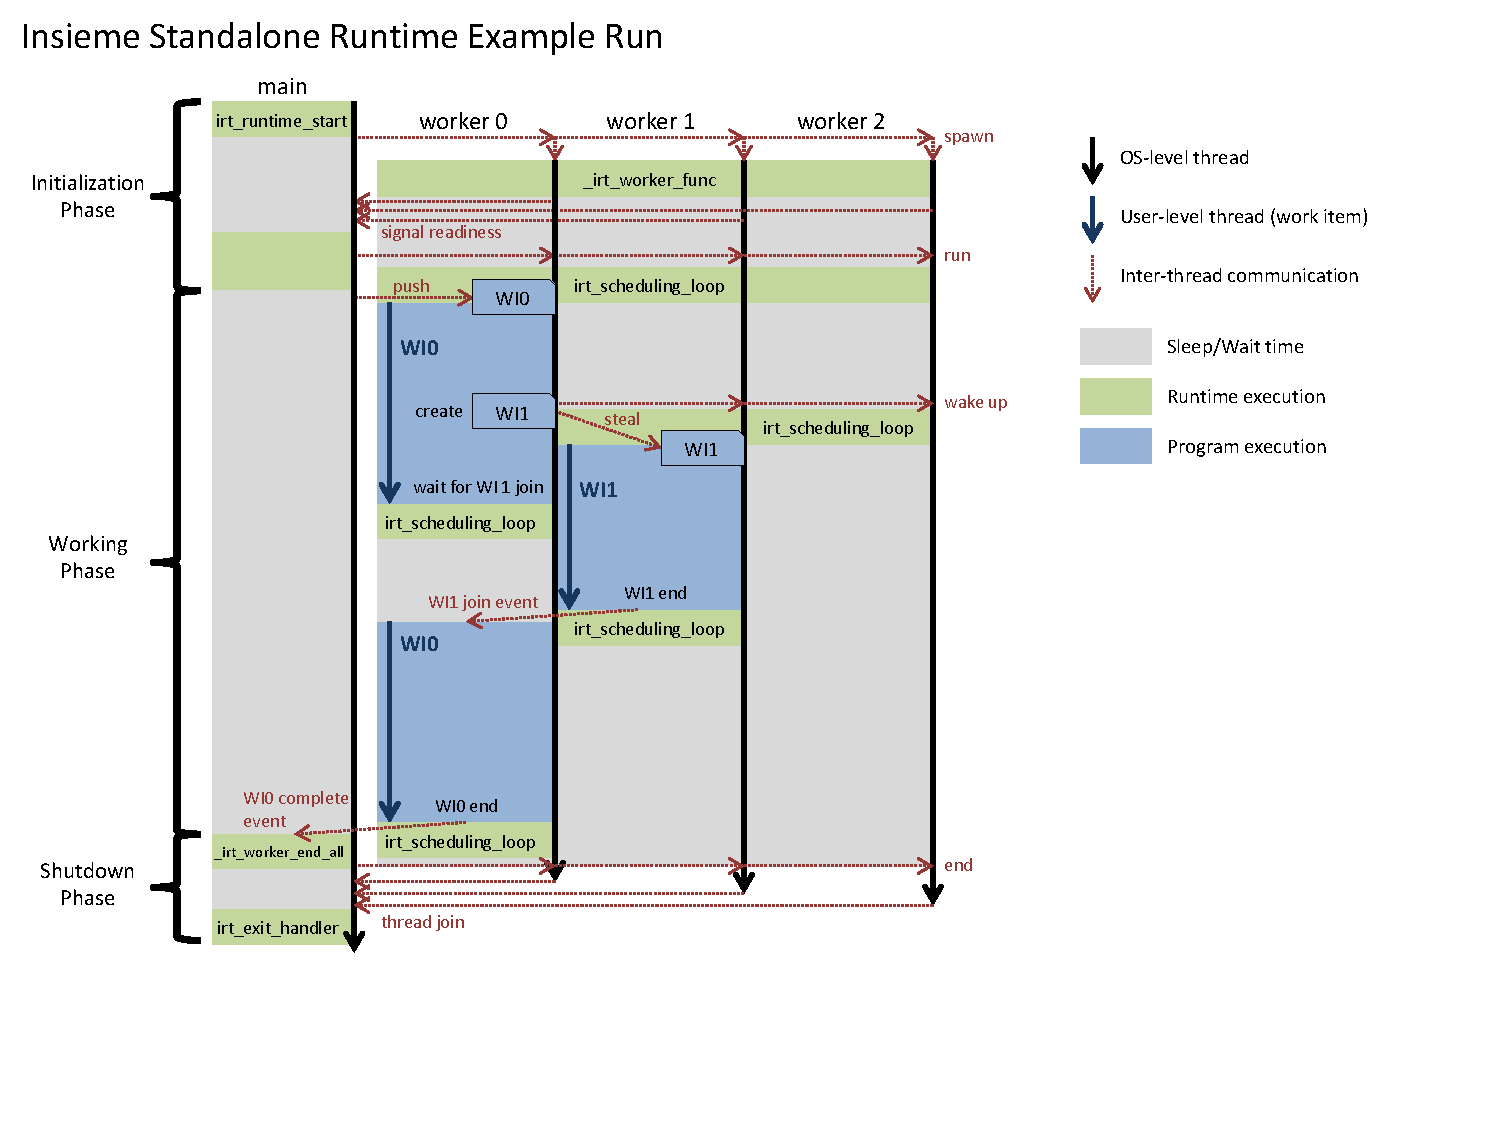
\includegraphics[width=\textwidth, trim=2cm 2cm 4cm 2cm]{pics/runtime/standalone_runtime_run.pdf}
	\caption{Timeline of a simple execution of the standalone runtime}
	\label{fig:runtime:execution}
\end{figure}


%%%%%%%%%%%%%%%%%%%%%%%%%%%%%%%%%%%%%%%%%%%%%%%%%%%%%%%%%%%%%%%%%%%%%%%%%%%%%%%
%%%%%%%%%%%%%%%%%%%%%%%%%%%%%%%%%%%%%%%%%%%%%%%%%%%%%%%%%%%%%%%%%%%%%%%%%%%%%%%
\section{Utilities}
\subsection{MinLWT -- Lightweight user-mode threads}
\subsection{Affinity}
\subsection{Error Handling}
\section{Workers}
\subsection{Scheduling}
\section{Work Items}
\section{Work Sharing}
\subsection{Loop Scheduling}
\section{Data Items}
\section{Event System}
\section{Instrumentation}
\section{Customizing the Runtime}
